\documentclass[conference]{IEEEtran}
\IEEEoverridecommandlockouts

\usepackage{cite}
\usepackage{amsmath,amssymb,amsfonts}
\usepackage{graphicx}
\usepackage{textcomp}
\usepackage{xcolor}
\usepackage{booktabs}
\usepackage{hyperref}

\def\BibTeX{{\rm B\kern-.05em{\sc i\kern-.025em b}\kern-.08em
    T\kern-.1667em\lower.7ex\hbox{E}\kern-.125emX}}

\begin{document}

\title{Visual Inspection System for Quadruped Robots Based on Large Language Models With a Human-in-the-Loop Mechanism}

\author{
\IEEEauthorblockN{Muhamad Rizano Alamsyah}
\IEEEauthorblockA{
\textit{Department of Computer Engineering}\\
\textit{Institut Teknologi Sepuluh Nopember}\\
Surabaya, Indonesia\\
ershanoano@email.com}
\and
\IEEEauthorblockN{Muhtadin, S.T., M.T.}
\IEEEauthorblockA{
\textit{Department of Computer Engineering}\\
\textit{Institut Teknologi Sepuluh Nopember}\\
Surabaya, Indonesia\\
muhtadin@its.ac.id}
\and
\IEEEauthorblockN{Ir. Hany Boedinugroho, M.T.}
\IEEEauthorblockA{
\textit{Department of Computer Engineering}\\
\textit{Institut Teknologi Sepuluh Nopember}\\
Surabaya, Indonesia\\
hanny@its.ac.id}
}

\maketitle

\begin{abstract}
This research aims to integrate a Multimodal Large Language Model (MLLM) agent with the Jueying Lite3 robot to automate navigation and visual analysis, while designing a Human-in-the-Loop (HITL) architecture to ensure system adaptability mid-inspection mission. The system development utilizes the Model Context Protocol (MCP) standard and webhooks to connect natural language instructions with ROS Noetic navigation on the robot. Instructions are broken down into sequential sub-tasks requiring operator validation at each coordinate. At every inspection point, the robot captures an image of the object and compares it against Standard Operating Procedure (SOP) documents to assess condition compliance. Evaluation was conducted through isolated component testing (tool calling, image analysis, plan generation), end-to-end system testing, and operator workload measurement using the NASA-TLX questionnaire. In isolated testing, Gemini 3.1 Pro achieved a tool calling success rate of 98.61\% (71/72), visual analysis accuracy of 100\% (27/27), and plan route efficiency of 100\% (12/12). In end-to-end testing across 9 tiered mission scenarios (easy, medium, hard), Gemini 3.1 Pro recorded a visual analysis accuracy of 93.33\% (28/30 inspection points) and a route efficiency of 100\% (9/9 scenarios). The system also successfully accommodated all 4 tested operator intervention scenarios (initial plan alteration, mid-mission object addition, object cancellation and replacement, and manual secondary movement), while reducing the total NASA-TLX workload score from 54.13 (under teleoperation) to 18.40. The MLLM architecture coupled with the HITL mechanism is capable of adaptively handling varying inspection scenarios in terms of route differences and target object variations without code modifications, ensuring system adaptability mid-mission, and significantly alleviating operator cognitive load in autonomous inspections.
\end{abstract}

\begin{IEEEkeywords}
quadruped robot, large language model, agentic AI, human-in-the-loop, model context protocol, ROS, autonomous inspection
\end{IEEEkeywords}

% ─────────────────────────────────────────────────────────
\section{Introduction}

The rapid growth of autonomous mobile robotics—projected to reach USD 9.56 billion by 2030 \cite{GrandView2024}—reflects increasing demand for automation in high-risk industrial environments \cite{LookingGlass2024}. Quadruped robots have emerged as particularly capable platforms for such environments due to their superior terrain adaptability compared to wheeled alternatives \cite{fan2024review}. However, despite this mobility advantage, the practical deployment of quadruped robots for industrial inspection remains operationally challenging due to human-robot interaction bottlenecks.

Current inspection paradigms fall into two main categories. \textit{Teleoperation} reduces human risk but requires continuous operator attention to interpret raw telemetry and visual feeds simultaneously while issuing motor commands, slowing decision-making and causing mental fatigue \cite{rea2022still}. Conversely, \textit{fully autonomous} systems utilize deterministic navigation to pre-programmed waypoints, as demonstrated by Darmawan \cite{Darmawan2025}. Although such systems reduce navigation effort, they remain inflexible: conventional object detection models (e.g., YOLOv8) are restricted to pre-defined trained classes, and any modification to inspection scope or criteria requires code-level reprogramming (\textit{hard-coding}).

Initial attempts at integrating Large Language Models (LLMs) for robot control, such as that proposed by Mahendra \cite{Mahendra2024}, introduce natural language flexibility but rely on a non-interactive ``batch-execution'' paradigm where complete multi-step plans are generated and executed upfront without intermediate verification \cite{huang2022language}. This lack of step-by-step validation prevents operators from intervening, modifying plans, or confirming intermediate findings mid-mission in dynamic operational environments.

This paper addresses these limitations by proposing an integrated autonomous visual inspection system powered by a Multimodal Large Language Model (MLLM) operating as an agentic orchestrator with a stepwise Human-in-the-Loop (HITL) control architecture \cite{ravichandar2020recent}. The main contributions of this work are:
\begin{enumerate}
    \item A distributed agentic architecture connecting an MLLM to a ROS-based quadruped robot controller via the Model Context Protocol (MCP), enabling natural language command interpretation, autonomous navigation, and dynamic zero-shot visual SOP compliance analysis.
    \item A stepwise Human-in-the-Loop (HITL) mechanism using webhook callbacks that pauses execution after each robot action, requiring explicit operator validation before proceeding to subsequent mission steps.
    \item An Agentic Retrieval-Augmented Generation (Agentic RAG) pipeline that grounds MLLM decisions in structured operational data (waypoint coordinates and SOP documents) retrieved on demand from a ground-truth database.
\end{enumerate}

% ─────────────────────────────────────────────────────────
\section{Related Work}

This research builds upon and addresses the limitations of two primary antecedent systems in quadruped robotics for industrial inspection.

\subsection{Deterministic Autonomous Inspection}
Darmawan \cite{Darmawan2025} developed an autonomous monitoring system using a quadruped robot to estimate the position of overheating components in substations. The system successfully integrated thermal cameras with YOLOv8s object detection and utilized FastLIO2 for 3D SLAM mapping alongside a combination of Pure Pursuit and Braitenberg algorithms for autonomous navigation. While highly reliable in execution, the system's navigation was fundamentally deterministic. The robot could only navigate to explicitly hard-coded coordinates, offering no flexibility to adapt to dynamic scenarios or semantic human instructions without code-level reprogramming by technical personnel. Furthermore, the reliance on manual telemetry monitoring continued to impose a high cognitive load on operators.

\subsection{LLM-Based Movement Planning}
To introduce semantic flexibility, Mahendra \cite{Mahendra2024} implemented a natural language interaction system using Google Gemini to autonomously generate movement plans for the Jueying Lite3 quadruped robot. The LLM parsed user commands into a complete JSON sequence of navigation actions which were then executed by the ROS Navigation Stack. However, the system utilized a ``batch-execution'' paradigm: the entire multi-waypoint plan was generated upfront and executed sequentially without interruption. This architecture lacked a step-by-step validation mechanism, stripping operators of the ability to intervene, modify the plan mid-mission, or verify intermediate inspection results before the robot proceeded to the next target.

\subsection{Proposed Contribution}
To bridge the gap between flexible language understanding and safe, interactive execution, our work introduces an agentic architecture via the Model Context Protocol (MCP). Unlike \cite{Mahendra2024}, our system does not generate a static sequence of actions. Instead, the LLM agent iteratively invokes robotic tools and evaluates their outcomes. By architecturally enforcing a stepwise Human-in-the-Loop mechanism, operators can validate or alter the inspection trajectory after every waypoint, while a Agentic Retrieval-Augmented Generation pipeline ensures the LLM's decisions are grounded in structured operational data.

% ─────────────────────────────────────────────────────────
\section{System Architecture}

\subsection{Overview}
The system is designed to bridge the communication gap between human operators and a quadruped robot through a natural language interface. Unlike conventional teleoperation that relies on full manual control, this system places a Multimodal Large Language Model (MLLM) as the central logic unit that orchestrates the information flow from user instructions to physical robot execution. The system adopts a distributed architecture comprising several loosely coupled components, as illustrated in Fig.~\ref{fig:architecture}. Communication between components follows explicit protocols to ensure modularity and replaceability.

\begin{figure*}[t!]
\centering
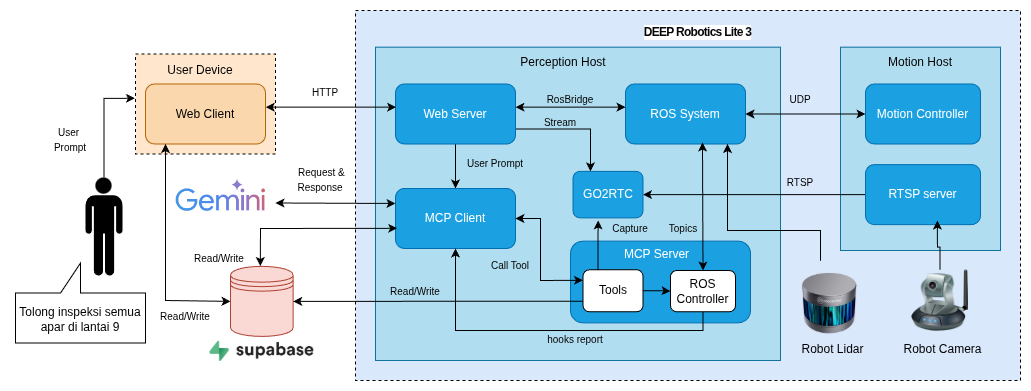
\includegraphics[width=\textwidth]{figures/arsitektur_new.png}
\caption{System architecture diagram showing the distributed components and their communication pathways. The LLM agent (MCP Client) bridges the operator interface and the robot-side MCP Server via the Model Context Protocol.}
\label{fig:architecture}
\end{figure*}

\subsection{Component Description}

\subsubsection{Google Gemini API}
Google Gemini API serves as the brain of the inspection system. Gemini processes natural language commands sent by the operator through the Web Client and analyzes them to formulate inspection plans. Using its \textit{function calling} feature, Gemini accesses various tools available on the MCP Server, deciding when to move the robot, when to capture images, or when to retrieve SOP documents from the database. Gemini API also performs visual analysis during inspection: when the robot camera captures an image, it is sent to Gemini alongside SOP instructions, and the model compares the visual condition of the object against the written standards.

\subsubsection{Supabase}
Supabase serves as a Backend-as-a-Service (BaaS) platform providing two primary functions. First, it acts as a relational database storing inspection target locations and coordinates, as well as session history containing conversation logs between the operator and Gemini to maintain mission context. Second, it provides cloud storage for SOP documents and every image captured by the robot camera during the inspection process.

\subsubsection{Web Dashboard}
The Web Dashboard is a Next.js application serving as the primary operator control station. It communicates with the backend via REST API for chat and data management. Real-time telemetry (robot pose, battery level, occupancy map, and LiDAR scan) is streamed directly from the ROS ecosystem via \textit{rosbridge} WebSocket. Camera video is delivered over WebRTC through go2rtc.

\subsubsection{MCP Client (LLM Agent)}
The MCP Client is a FastAPI service that acts as the agentic middleware. It holds the system prompt defining the inspection workflow, manages conversation history in Supabase, and implements the agentic loop: forwarding prompts to Gemini, intercepting \textit{function\_call} responses, dispatching tool calls to the MCP Server via MCP over HTTP, and injecting results back into the LLM context. The client also manages the system prompt containing personality configuration and operational constraints that Gemini must follow during missions.

\subsubsection{MCP Server}
The MCP Server is a FastMCP HTTP server running on the robot's onboard AI computer. It operates as a local abstraction layer that exposes all robot functionality as a collection of tools. These tools enable the LLM to move the robot by leveraging ROS functionality, search for waypoint coordinates, capture images from the robot camera, retrieve SOP documents, and perform visual analysis. The server also implements a webhook mechanism to send completion status back to the MCP Client after robot movements finish.

\subsubsection{ROS System}
ROS manages all communication and navigation tasks on the robot. It processes raw data from the robot's LiDAR sensor to generate environment maps and determine the robot's position accurately during missions. All physical movement coordination is managed through UDP connections to the Motion Host. RosBridge provides WebSocket connectivity that allows the web interface to access robot telemetry data.

\subsubsection{Motion Controller}
The Motion Controller is the lowest-level control unit that interfaces directly with the Jueying Lite3 hardware. It handles dynamic balance and actuator joint rotation (\textit{gait planning}), converting abstract velocity commands from ROS into motor torque signals that physically move the robot.

\subsubsection{Video Streaming (GO2RTC and RTSP)}
GO2RTC manages the distribution of visual data from the robot camera to various system modules, receiving data streams via RTSP from the RTSP server connected directly to the camera hardware on the Motion Host. The RTSP server provides raw video data access through the Real-Time Streaming Protocol.

\subsection{Communication Protocols}
Table~\ref{tab:protocols} summarizes the inter-component communication pathways and protocols used throughout the system.

\begin{table}[htbp]
\caption{Communication Protocols Between System Components}
\label{tab:protocols}
\centering
\resizebox{\columnwidth}{!}{%
\begin{tabular}{lll}
\toprule
\textbf{Link} & \textbf{Protocol} & \textbf{Purpose} \\
\midrule
Web $\leftrightarrow$ Backend & REST / HTTP & Chat messages, CRUD \\
Web $\leftrightarrow$ ROS & WebSocket (rosbridge) & Telemetry, maps, LiDAR \\
Web $\leftrightarrow$ Robot camera & WebRTC (go2rtc) & Live video feed \\
Backend $\leftrightarrow$ MCP Server & MCP over HTTP/SSE & Tool invocation \\
MCP Server $\leftrightarrow$ ROS & rospy (topics/actions) & cmd\_vel, move\_base \\
Robot $\rightarrow$ Backend & HTTP POST (webhook) & Navigation completion \\
Backend $\leftrightarrow$ Gemini & Google GenAI SDK & LLM inference \\
All $\leftrightarrow$ Supabase & REST API / SDK & Database \& storage \\
ROS $\leftrightarrow$ Motion Host & UDP & Velocity commands \\
Camera $\rightarrow$ GO2RTC & RTSP & Video stream \\
\bottomrule
\end{tabular}%
}
\end{table}

\subsection{Hardware Platform}
The robot platform is the DEEPRobotics Jueying Lite3 Pro \cite{DEEPRoboticsLite3Pro2024}, a 12-DOF quadruped (mass 12.7 kg, 610$\times$370$\times$445 mm standing), augmented with a Leishen C16 16-channel 3D LiDAR \cite{DEEPRoboticsLite3LiDAR2025}. The onboard AI computer is an NVIDIA Jetson Xavier NX, which runs all software components (ROS stack, MCP Server, MCP Client, and web application) as a single-host deployment managed by \textit{systemd} services and Docker Compose. Remote access is provided through Tailscale VPN, eliminating the need for a shared local network.

% ─────────────────────────────────────────────────────────
\section{System Design}

\subsection{System Workflow}
The operational workflow of the autonomous visual inspection system is structured into three main phases executed sequentially across five primary system actors: the Human Operator, the AI Agent (MCP Client), the MCP Server, the Supabase BaaS Database, and the Quadruped Robot (ROS \& Camera), as illustrated in Fig.~\ref{fig:sequence}.

\begin{figure*}[t!]
\centering
\includegraphics[width=0.8\textwidth]{figures/alur_baru.png}
\caption{Sequence diagram depicting the multi-actor system interaction across three phases: (1) Context Retrieval \& Planning, (2) Stepwise Autonomous Execution \& Analysis, and (3) HITL Validation \& Reporting.}
\label{fig:sequence}
\end{figure*}

\subsubsection{Planning Phase}
The first phase focuses on parsing abstract natural language instructions from the operator and formulating a grounded inspection plan prior to physical robot movement. Upon receiving an operator prompt via the web chat panel, the AI Agent executes Agentic RAG context retrieval by calling MCP tools (\texttt{get\_sop\_file} and \texttt{get\_object\_waypoints}). The MCP Server queries Supabase to retrieve spatial coordinates and SOP document metadata. Grounded in this data, the AI Agent generates a structured inspection plan ordered by nearest waypoint priority and presents it on the dashboard. The system then enters a Human-in-the-Loop control gate, requiring explicit operator confirmation before physical execution commences.

\subsubsection{Execution and Analysis Phase}
Once approved, the AI Agent commands the MCP Server to invoke \texttt{async\_navigate\_to\_waypoint} for the first target. The MCP Server dispatches the goal to the ROS Navigation Stack and immediately returns a ``running'' status, preventing the LLM context from blocking during physical transit. When the robot reaches the target coordinates, ROS triggers a webhook callback from the MCP Server to the AI Agent. Upon receiving arrival feedback, the AI Agent automatically invokes \texttt{capture\_and\_inspect\_image}. The MCP Server captures a camera frame via go2rtc, crops the target object, evaluates visual SOP compliance using Gemini, uploads the processed image to Supabase Storage, and returns a public URL alongside structured findings.

\subsubsection{Reporting and HITL Validation Phase}
The final phase reports findings to the operator and determines mission progression. The AI Agent displays visual inspection results and cropped images on the chat panel. The workflow then branches based on operator feedback: if the operator identifies an anomaly or issues an interruption command (e.g., requesting a closer view), the AI Agent executes immediate tool calls (e.g., \texttt{async\_move}) to fulfill the request. If the result is approved, the operator confirms to proceed, prompting the AI Agent to navigate to the next target waypoint. This cycle repeats until all plan items are completed.

\subsection{MCP Tool Definitions}
The MCP Server exposes eight tools that collectively span the full capability surface of the robot, as detailed in Table~\ref{tab:tools}. Tool schemas are converted from MCP format to Gemini \textit{FunctionDeclaration} format at runtime by the MCP Client.

\begin{table}[htbp]
\caption{MCP Tools Exposed by the Robot Server}
\label{tab:tools}
\centering
\resizebox{\columnwidth}{!}{%
\begin{tabular}{lp{5cm}}
\toprule
\textbf{Tool} & \textbf{Description} \\
\midrule
\texttt{async\_move} & Open-loop velocity control. Accepts linear speed (m/s), angular speed (rad/s), and duration (s). Returns ``running'' immediately. \\
\texttt{async\_navigate\_to\_waypoint} & Autonomous navigation via \textit{move\_base} Action. Accepts (x, y, yaw). Returns ``running'' and fires webhook on arrival. \\
\texttt{toggle\_sit\_stand} & Sends binary command 0x21010202 to transition robot posture between sitting and standing. \\
\texttt{look\_up\_down} & Adjusts body pitch angle (range $\pm$32767) for a specified duration to tilt the camera view up or down. \\
\texttt{get\_object\_waypoints} & Hierarchical DB query: searches objects by keyword across maps $\rightarrow$ locations $\rightarrow$ sub-locations $\rightarrow$ waypoints, returning structured coordinate data. \\
\texttt{get\_sop\_file} & Retrieves SOP document metadata and URL links from Supabase. Downloads and text extraction are handled by MCP Client. \\
\texttt{capture\_and\_inspect\_image} & Captures a frame via go2rtc snapshot, uses Gemini to detect and crop the target object, analyzes against SOP, uploads to Supabase, and returns analysis results. \\
\texttt{say\_hello} & Greeting and conversational response tool. \\
\bottomrule
\end{tabular}%
}
\end{table}

\subsection{Agentic Loop Processing}
The reasoning cycle of the agent is managed within the main processing loop. During execution, the Gemini model may call multiple control functions sequentially within a single conversation turn. However, if the model calls an asynchronous navigation function that returns a ``running'' status, the client immediately halts the language model's reasoning loop, saves all state to the database, and directly returns a waiting status response to the operator without blocking the server execution thread. The next reasoning cycle is triggered as a new request after the system receives callback data from the robot system marked with ``[ROBOT\_FEEDBACK]'' text, indicating the robot has arrived at the destination.

This mechanism ensures that long-running physical operations (e.g., 30-second navigation) do not block the server. The webhook-driven architecture decouples LLM inference from robot execution time, enabling the system to remain responsive even during extended autonomous operations.

\subsection{RAG-Based Operational Grounding}
Rather than encoding inspection knowledge in the system prompt, the architecture uses tool-time retrieval (Agentic RAG). When Gemini identifies an inspection target, it calls \texttt{get\_object\_waypoints} to fetch spatial coordinates from the database and \texttt{get\_sop\_file} to retrieve the relevant SOP document. This approach ensures that: (1) the LLM always operates on the latest operational data without redeployment; (2) inspection procedures can be updated by operators uploading new SOP files without modifying any code; and (3) hallucination risk is reduced as spatial data is retrieved from a ground-truth database rather than generated.

\subsection{Navigation Stack}
The ROS Navigation Stack is configured with a global planner for shortest route computation and a Timed Elastic Band (TEB) local planner \cite{rosmann2012trajectory} for real-time obstacle avoidance. Localization is performed by HDL Localization using NDT scan matching \cite{biber2003normal} combined with Fast-GICP \cite{koide2021voxelized} against a 3D point cloud map built by Faster-LIO (LiDAR-Inertial Odometry). The 3D map is projected to a 2D occupancy grid for use by the Navigation Stack's costmap.

% ─────────────────────────────────────────────────────────
\section{Implementation}

\subsection{Deployment}
All software components are deployed on the robot's Jetson Xavier NX. Four \textit{systemd} services manage the core stack: LiDAR driver, navigation (\textit{move\_base} + localization), MCP Server (port 8001), and MCP Client/Backend (port 8082). The web dashboard runs in a Docker Compose container (port 3000). Tailscale VPN provides a stable overlay network; the Supabase instance runs on a separate server, mimicking a cloud deployment without public infrastructure requirements.

\subsection{MCP Client Implementation}
The MCP Client is built using Python with FastAPI as the core framework, providing high-performance asynchronous HTTP request handling. On Linux, the implementation uses \texttt{uvloop} as an asynchronous event loop replacement to maximize data transfer throughput. The primary entry point is the \texttt{POST /api/chat\_robot} endpoint, which receives requests containing conversation session IDs, operator prompts, model selections, and real-time telemetry metadata. Cross-Origin Resource Sharing (CORS) policies restrict access strictly to the local web application.

\subsubsection{Session Management}
Conversation session management stores all inspection activities into the \texttt{chat-sessions} and \texttt{chat-messages} tables in Supabase. Every new user message, final model text response, internal function call, and tool execution result are stored sequentially. Since Gemini API message structures are complex objects, the MCP Client serializes them into JSONB format for persistent database storage. A status column in the database table serves as a message filter marker, where internal function call logs and raw tool responses are given special flag values so they are not displayed on the user chat panel.

\subsubsection{Context Re-injection}
A significant implementation challenge involves maintaining multimodal context across stateless LLM API calls. When historical conversations are loaded from the database, the client implements a context re-injection mechanism: any previously retrieved SOP documents or captured images are re-downloaded from Supabase Storage. For PDF documents and JPEG images, the binary data is directly converted to byte array objects and injected as \texttt{Part.from\_bytes} into the Gemini input message list. For DOCX documents, the client uses the \texttt{python-docx} library to extract all paragraph text first and inject it as plain text message parts, ensuring the language model can read SOP compliance rules in full without losing context.

\subsubsection{Schema Conversion}
The MCP Client connects to the MCP Server via HTTP transport using FastMCP. Upon connection, the client requests the list of supported functions. Since FastMCP input parameter schemas are not compatible with Gemini API specifications, the client performs recursive schema conversion by stripping unsupported \texttt{title} and \texttt{additionalProperties} fields before wrapping them into Gemini \texttt{FunctionDeclaration} objects. This prevents function registration failures on the Gemini API.

\subsection{System Prompt Engineering}
The system prompt is structured into five key sections that define the agent's behavior:
\begin{enumerate}
    \item \textbf{Role Definition:} Defines the AI as a quadruped inspection robot assistant with explicit responsibilities for planning, tool-based robot control, and transparent operator interaction.
    \item \textbf{Main Workflow:} Instructs the agent to retrieve coordinates and SOP data, formulate a shortest-distance inspection plan, present it to the operator, and \textit{wait for explicit approval}. Each plan point follows a mandatory sub-step sequence: stand $\rightarrow$ navigate $\rightarrow$ capture and inspect $\rightarrow$ report. Points are executed one at a time; between points, the operator is asked whether to continue, modify, or stop.
    \item \textbf{Asynchronous Tool Handling:} Tools prefixed with \texttt{async\_} return ``running'' immediately. The agent must halt all tool calls upon receiving this status and wait for the ``[ROBOT\_FEEDBACK]'' signal. Upon receiving arrival feedback, the agent must immediately invoke the image capture tool without waiting for operator instruction.
    \item \textbf{Movement Safety:} When the operator requests the robot to move closer, the agent advances 0.3m per step and records total additional distance. Before proceeding to the next waypoint, a reverse movement equal to the total additional distance plus 0.1m margin is mandatory to prevent navigation drift accumulation.
    \item \textbf{Operational Constraints:} Robot status metadata is distinguished from user instructions. The agent must prioritize physical safety, avoid aggressive movements, never execute plans without operator approval, and always invoke tools rather than merely describing intended actions.
\end{enumerate}

\subsection{MCP Server Implementation}
The MCP Server is built using FastMCP in Python, running directly on the robot's onboard computer. Each registered tool is decorated with special annotations so that input schemas and function descriptions are automatically sent to the client upon connection.

The \texttt{capture\_and\_inspect\_image} tool implements a multi-stage pipeline: (1) capture a raw frame from the robot camera via go2rtc snapshot protocol; (2) send the image to Gemini with object detection instructions to obtain normalized bounding box coordinates; (3) crop the image using OpenCV based on detected coordinates with a 20\% margin to center the target object; (4) if SOP text is available, perform visual compliance analysis comparing the cropped image against SOP criteria, returning a status of \textit{normal}, \textit{abnormal}, or \textit{inconclusive}; and (5) upload the processed image to Supabase Storage and return the public URL along with structured analysis data.

For asynchronous tools (\texttt{async\_move} and \texttt{async\_navigate\_to\_waypoint}), the server publishes velocity commands or navigation goals to ROS topics and immediately returns a ``running'' status. Upon goal completion, the ROS action server triggers an HTTP POST webhook callback to the MCP Client, carrying the arrival status message.

\subsection{Web Dashboard}
The operator dashboard (Fig.~\ref{fig:dashboard}) is a single-page Next.js application with TypeScript, utilizing TanStack React Query for state synchronization and caching. Navigation stack initialization and shutdown scripts are managed via server-side API routes (\texttt{/api/shell}).

\begin{figure}[htbp]
\centering
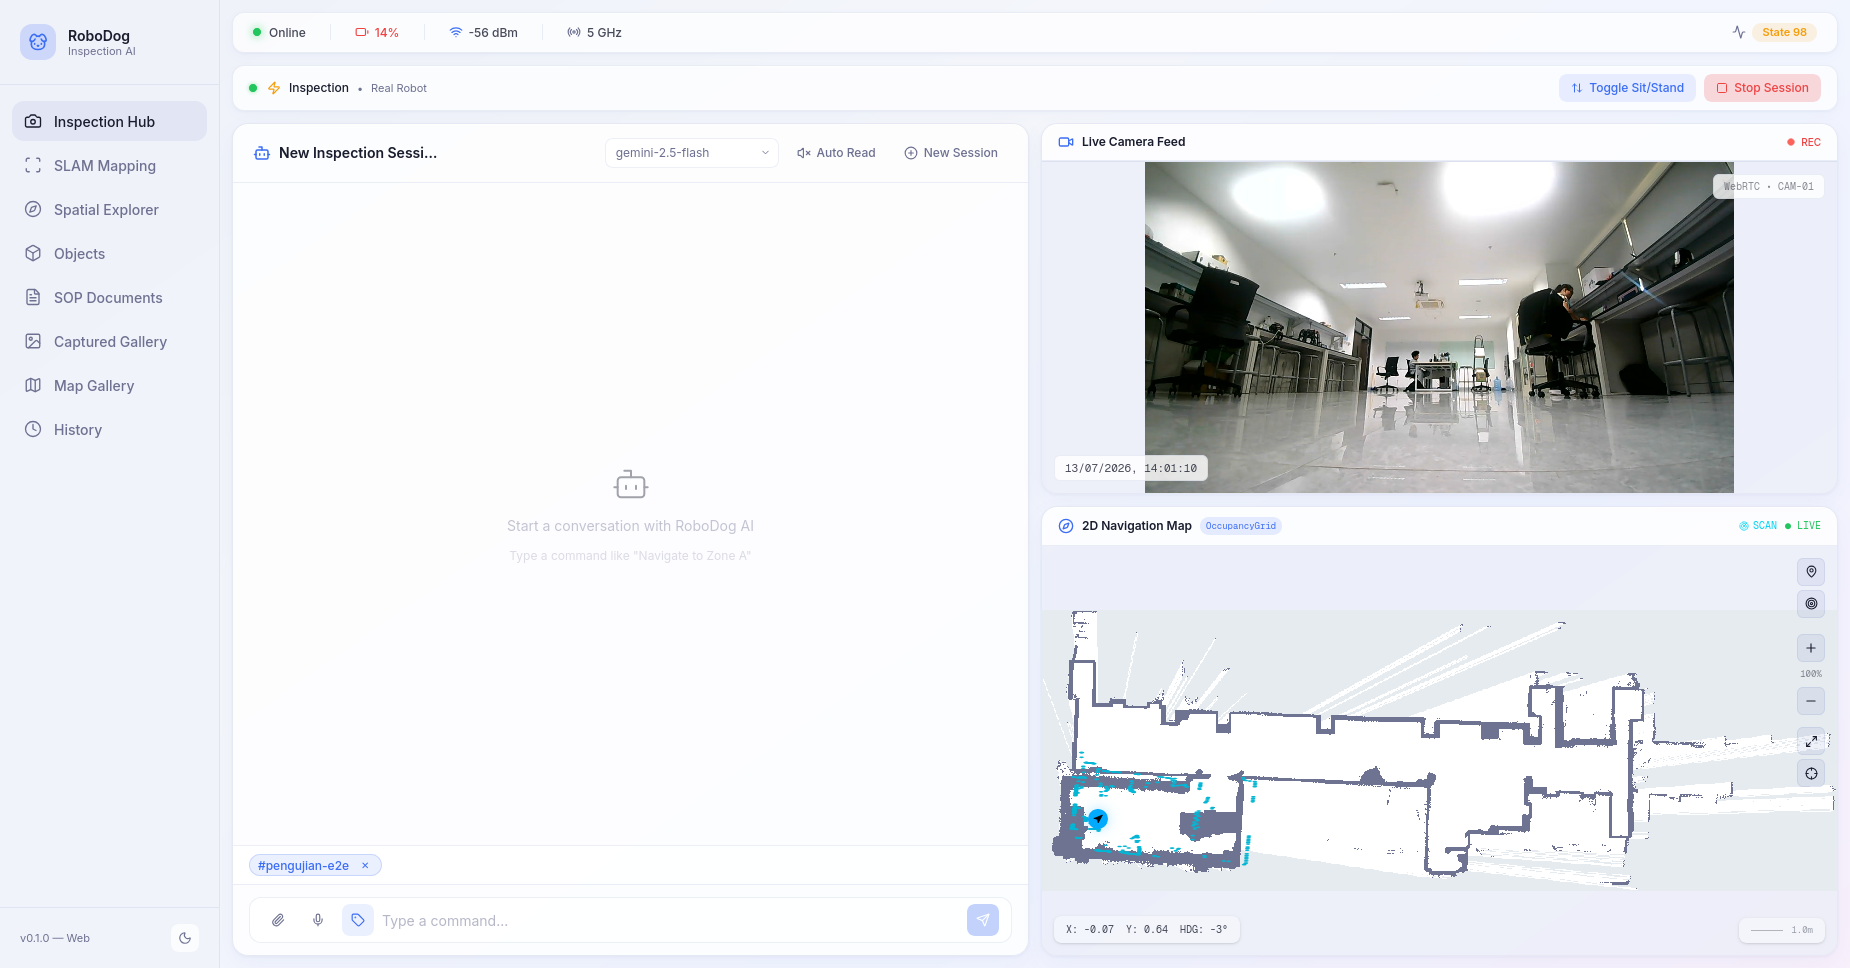
\includegraphics[width=\columnwidth]{figures/inspection_hub.png}
\caption{Web dashboard Inspection Hub: split-screen layout with LLM chat panel (left) and real-time navigation map alongside video feed (right).}
\label{fig:dashboard}
\end{figure}

The primary \textit{Inspection Hub} page features a split-screen layout. The left panel provides the LLM chat interface with model selection (Gemini 3.1 Pro Preview, Gemini 2.5 Flash, Qwen 3.5 27B). Every operator message automatically includes real-time robot telemetry from RosBridge WebSocket topics: battery level (\texttt{/battery\_level}), motion status (\texttt{/robot\_basic\_state}), and position coordinates (\texttt{/odom}). The chat subscribes to Supabase Realtime channel on the \texttt{chat-messages} table, enabling instant rendering of new messages including tool call logs without page reload.

The right panel displays a live video feed via WebRTC (go2rtc) and a real-time 2D navigation map. The map processes OccupancyGrid data from the \texttt{/map} topic, renders robot position from \texttt{/odom}, LiDAR scan points from \texttt{/scan}, and the global navigation path from \texttt{/move\_base/GlobalPlanner/plan} as a dashed yellow line. Operators can set initial pose estimates (\texttt{/initialpose}) and navigation goals (\texttt{/move\_base\_simple/goal}) directly on the map via drag interaction.

An active session bar at the top provides a Sit/Stand toggle button (publishing command code \texttt{0x21010202} to \texttt{/simple\_cmd}) and a Stop Session button that triggers \texttt{stop\_nav.sh} via \texttt{/api/shell}, disconnects WebSockets, and stops the periodic heartbeat signal (\texttt{0x21040001} at 2 Hz) to prevent the robot from entering loss-of-control protection mode.

Supporting pages include: \textit{Spatial Explorer} for hierarchical management across \texttt{maps} $\rightarrow$ \texttt{locations} $\rightarrow$ \texttt{sub\_locations} $\rightarrow$ \texttt{object\_waypoints}; \textit{Object Manager} for defining inspection target categories with keywords and SOP associations; \textit{SOP Manager} for drag-and-drop uploading of procedure documents with unique timestamp prefixes; \textit{Capture Gallery} for browsing and downloading images; and \textit{Session History} featuring a slide-out panel for reviewing past conversation logs.

\subsection{Database Schema}
The Supabase PostgreSQL database uses a relational schema with seven main tables: \texttt{maps} (environment map metadata and YAML config paths), \texttt{locations} (hierarchical physical locations with parent\_id and optional arrival coordinates), \texttt{sub\_locations} (room-level sub-locations), \texttt{objects} (inspection target types with keyword arrays and SOP URL links), \texttt{object\_waypoints} (navigation view coordinates with x, y, yaw, and optional camera PTZ parameters), \texttt{chat-sessions} (conversation session metadata), and \texttt{chat-messages} (full message history with JSONB content and display filter flags). Supabase Storage provides two folders: \texttt{sop} for procedure documents and \texttt{captured} for robot camera images, both generating public URLs for display in the chat interface.

% ─────────────────────────────────────────────────────────
\section{Evaluation}

\subsection{Experimental Setup}
Experiments were conducted in an indoor laboratory environment replicating an industrial inspection scenario containing three types of inspection objects: fire extinguishers (APAR), electrical outlets, and trash cans. Each object was tested under normal and anomalous conditions (e.g., fire extinguisher lying on the floor, detached hose, damaged plug, scattered trash). All functional tests were performed on three LLM models: Gemini 3.1 Pro Preview (large-scale cloud model with advanced reasoning), Gemini 2.5 Flash (fastest and most cost-efficient cloud model), and Qwen 3.5 27B (locally hosted open-source model for future-proofing). The evaluation comprised four test categories: tool calling, visual analysis, route planning, and full end-to-end integration.

\subsection{Tool Calling and Intent Recognition}
The dataset consisted of 72 test cases covering 8 tool types across three difficulty levels: Level 1 (explicit commands naming the tool directly), Level 2 (implicit natural language without explicit tool names), and Level 3 (abstract contextual instructions requiring semantic reasoning). Each tool-level combination was tested 3 times, yielding $8 \times 3 \times 3 = 72$ cases per model.

\begin{table}[htbp]
\caption{Summary of Tool Calling Evaluation}
\label{tab:eval_tools}
\centering
\resizebox{\columnwidth}{!}{%
\begin{tabular}{lccc}
\toprule
\textbf{Metric} & \textbf{Gemini 2.5 Flash} & \textbf{Gemini 3.1 Pro} & \textbf{Qwen 3.5 27B} \\
\midrule
Success Rate & 93.06\% & 98.61\% & 88.89\% \\
Avg. Latency (s) & 2.03 & 4.11 & 2.96 \\
Avg. Total Tokens & 1,139 & 1,144 & 1,587 \\
\bottomrule
\end{tabular}%
}
\end{table}

Gemini 3.1 Pro achieved the highest success rate (98.61\%), with all failures concentrated on Level 3. All three models performed perfectly on Levels 1 and 2. The three tools that caused failures at Level 3 were \texttt{look\_up\_down}, \texttt{say\_hello}, and \texttt{toggle\_sit\_stand}, sharing the characteristic that abstract instructions did not mention robot actions directly. Failure patterns included: (1) models understanding context but choosing to describe actions rather than invoking tools; (2) models failing to associate the instruction with an available tool; and (3) models performing excessive planning before executing the required tool.

\begin{figure}[htbp]
\centering
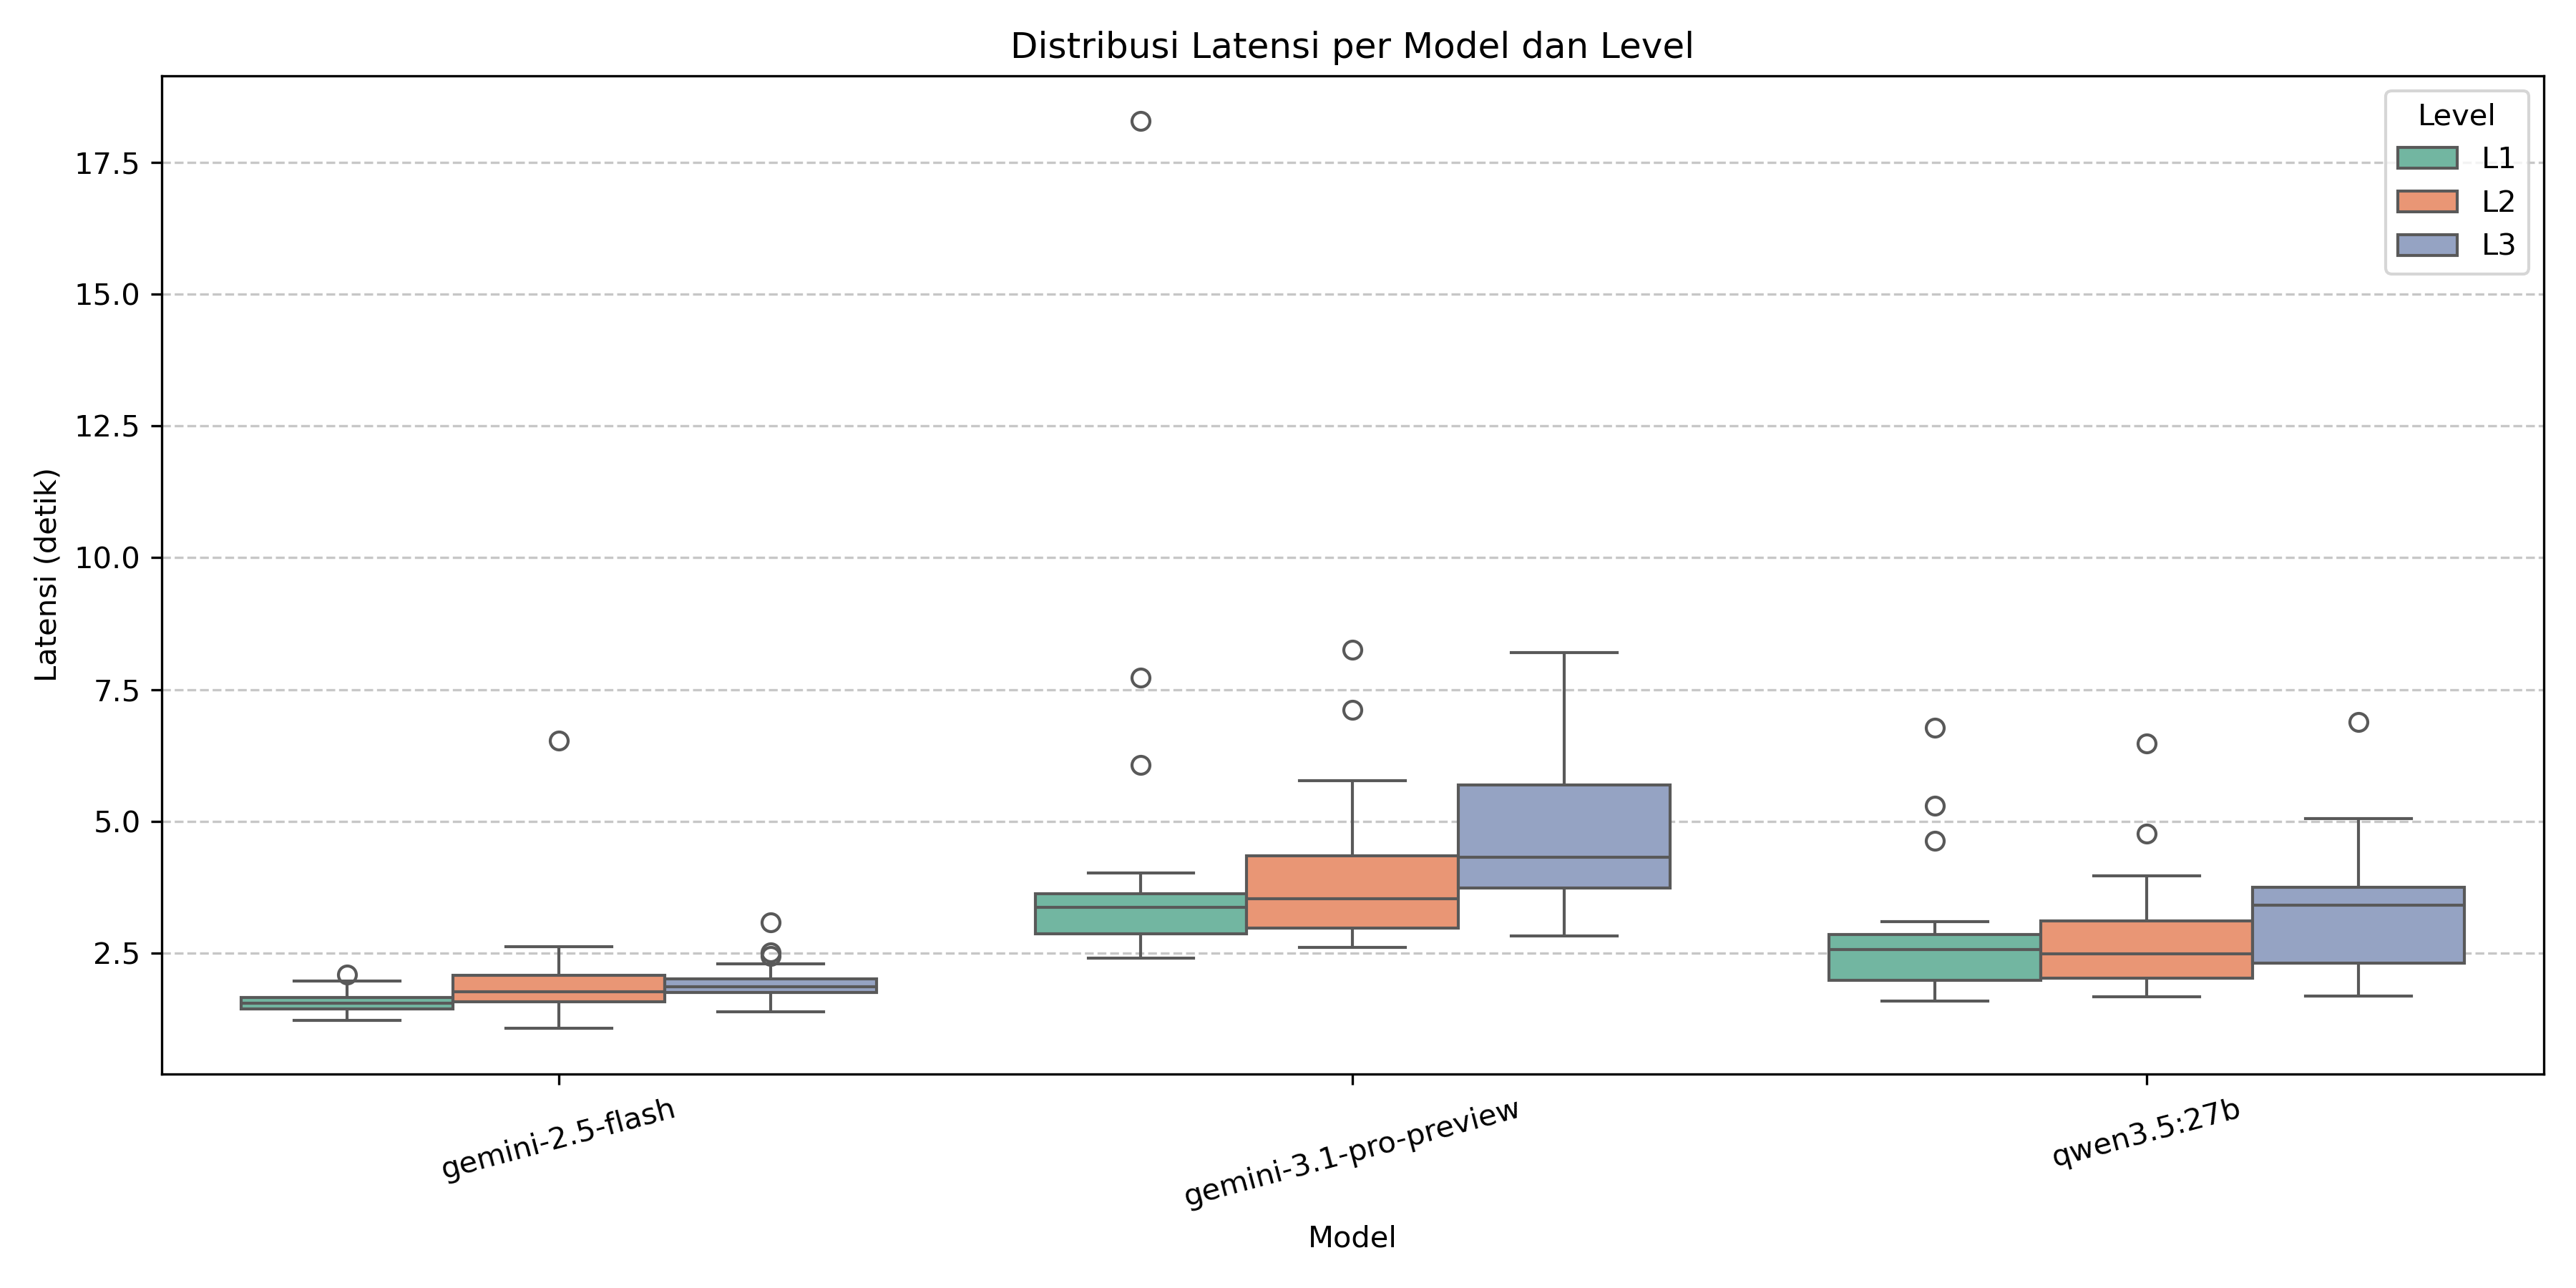
\includegraphics[width=\columnwidth]{figures/boxplot_tools_latensi.png}
\caption{Latency distribution for tool calling evaluation across three models. Gemini 2.5 Flash demonstrates the lowest median latency, while Gemini 3.1 Pro shows higher latency due to internal reasoning overhead.}
\label{fig:boxplot_tools}
\end{figure}

As shown in Fig.~\ref{fig:boxplot_tools}, Gemini 2.5 Flash maintained the shortest response time across all levels. Gemini 3.1 Pro recorded the highest latency due to its deeper internal reasoning mechanism, despite consuming nearly identical token counts to Flash. This confirms that latency is not solely determined by output length but by the complexity of internal reasoning processes.

\subsection{Multimodal Visual Analysis}
Visual inspection was evaluated across 3 object types $\times$ 3 conditions $\times$ 3 camera angles = 27 test cases per model. Each condition assessed the model's ability to cross-reference camera captures with retrieved SOP documents.

\begin{table}[htbp]
\caption{Summary of Visual Analysis Evaluation}
\label{tab:eval_visual}
\centering
\resizebox{\columnwidth}{!}{%
\begin{tabular}{lccc}
\toprule
\textbf{Metric} & \textbf{Gemini 2.5 Flash} & \textbf{Gemini 3.1 Pro} & \textbf{Qwen 3.5 27B} \\
\midrule
Success Rate & 85.19\% & 100.00\% & 85.19\% \\
Avg. Latency (s) & 9.62 & 19.31 & 35.29 \\
Avg. Total Tokens & 1,980 & 3,297 & 5,071 \\
\bottomrule
\end{tabular}%
}
\end{table}

Gemini 3.1 Pro achieved perfect 100\% accuracy across all object types and conditions, including the most challenging scenario: detecting a detached fire extinguisher hose. Gemini 2.5 Flash hallucinated on this scenario, incorrectly stating the hose was properly attached. Qwen 3.5 failed on color detection (misidentifying red extinguisher tubes as yellow due to dominant label sticker pixels) and spatial detail analysis. A common vulnerability was the ``detached hose'' scenario, which requires fine-grained spatial reasoning about component relationships.

\begin{figure}[htbp]
\centering
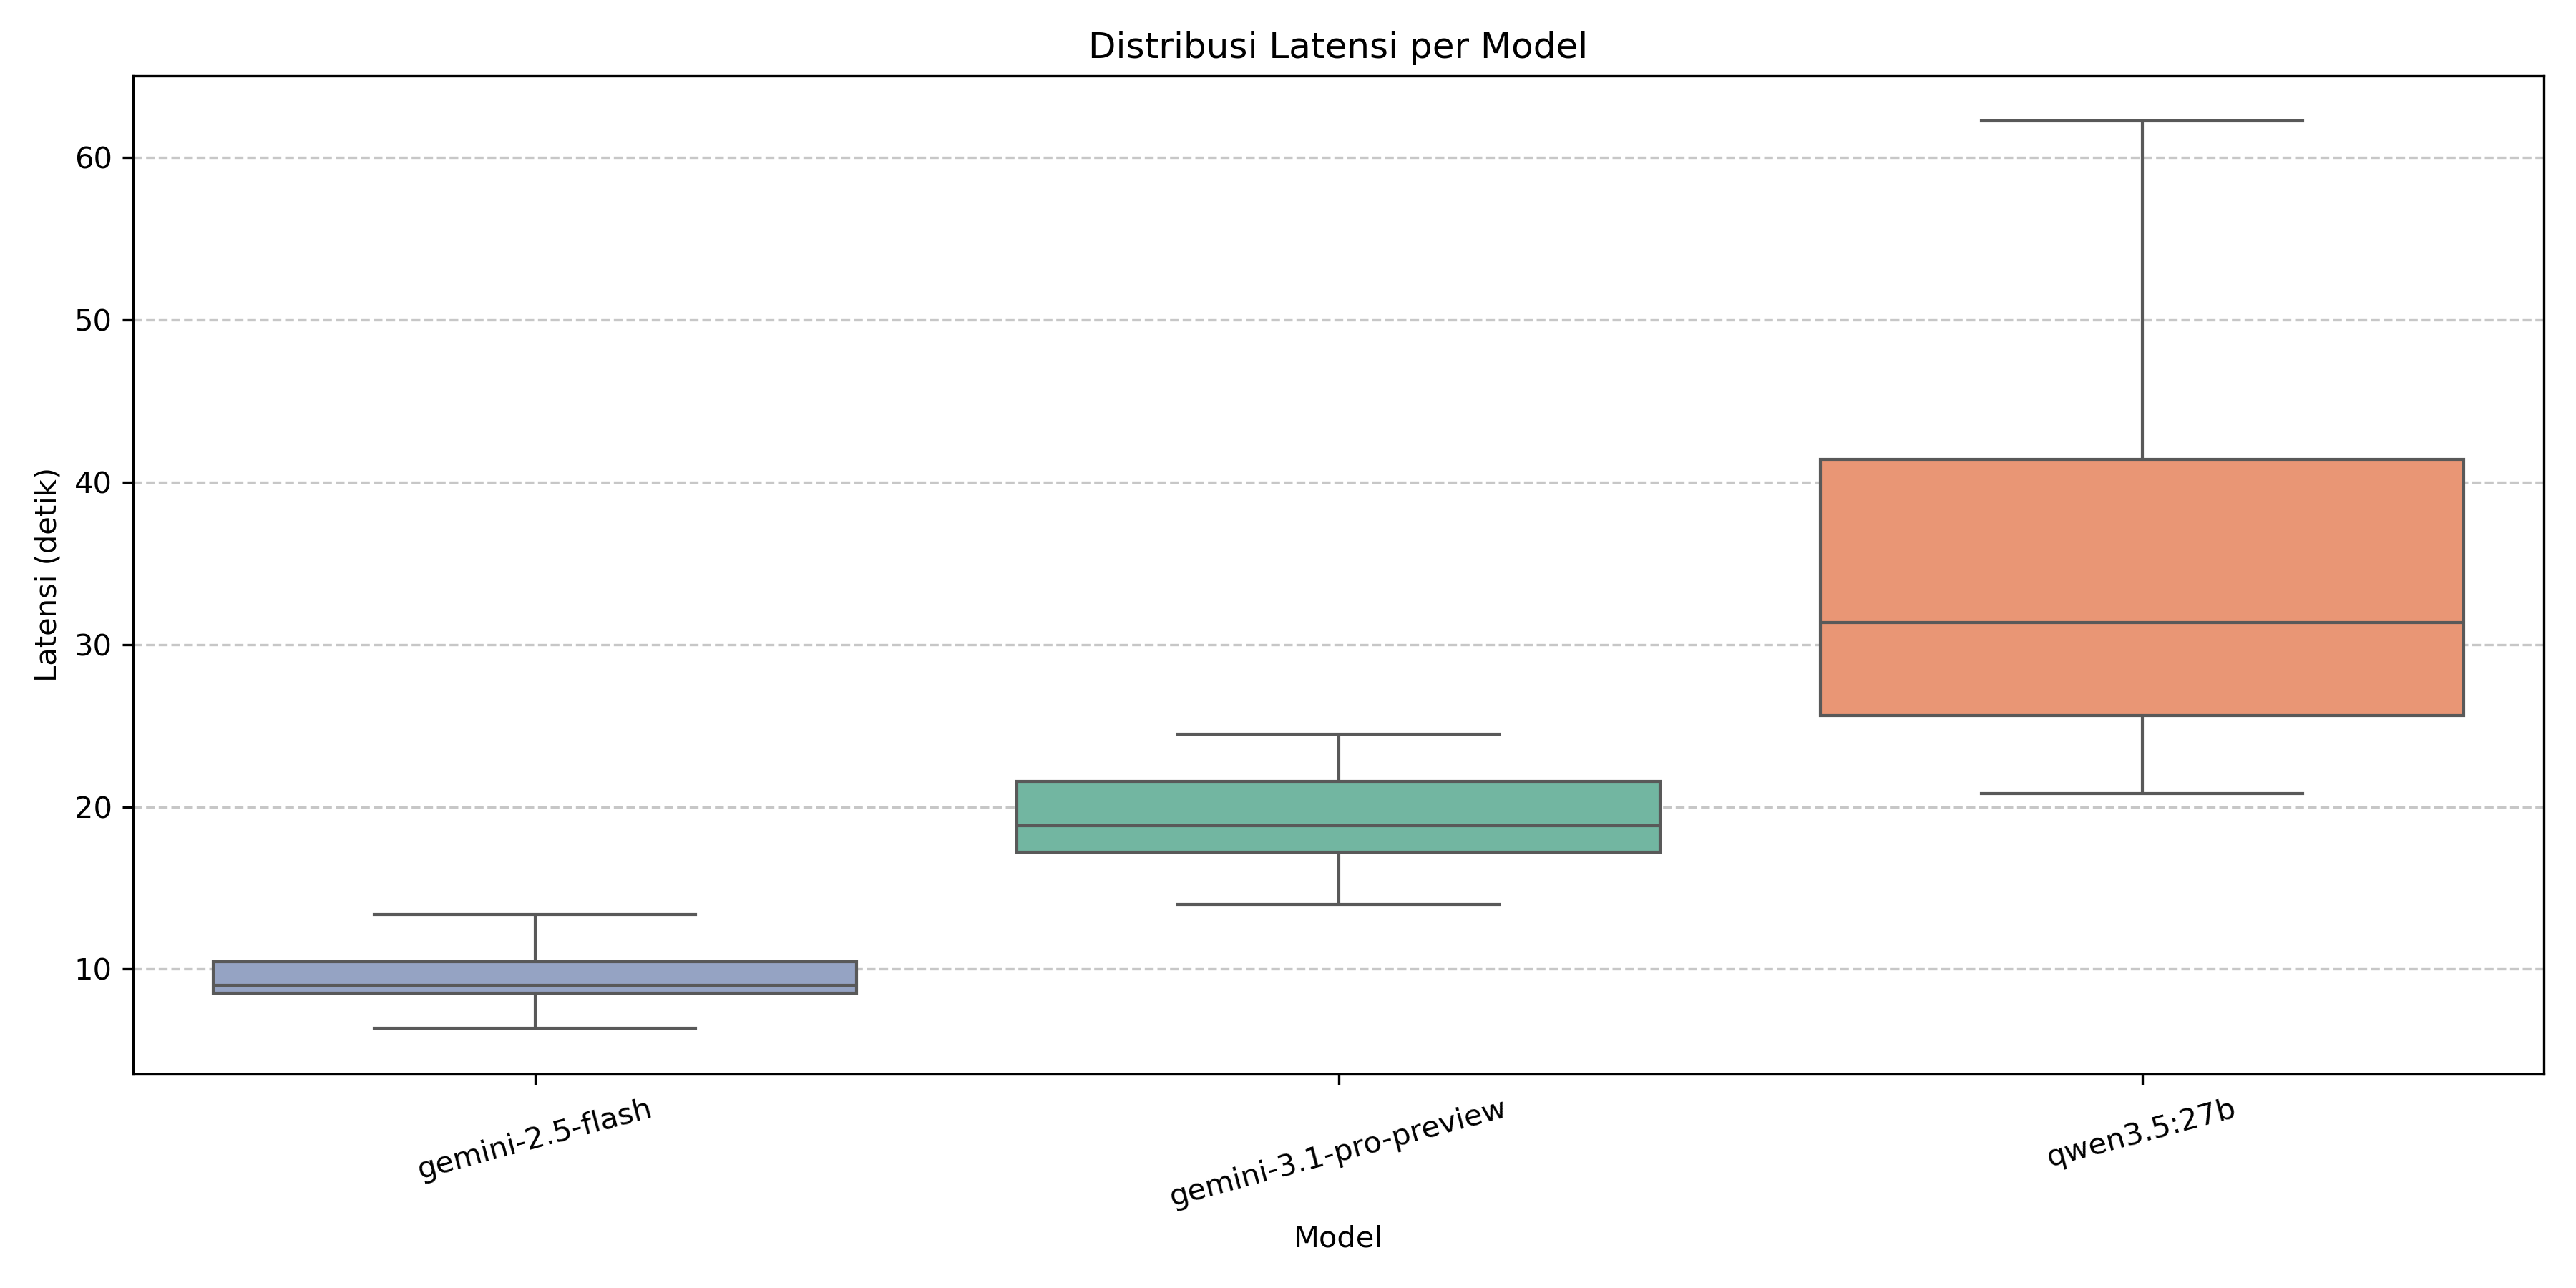
\includegraphics[width=\columnwidth]{figures/boxplot_inspeksi_latensi.png}
\caption{Latency distribution for visual analysis evaluation. Qwen 3.5 shows significantly higher latency due to local vision encoding overhead on the GPU server.}
\label{fig:boxplot_visual}
\end{figure}

Fig.~\ref{fig:boxplot_visual} reveals a significant trend reversal: Qwen 3.5, which was competitive on text-only tool calling, exhibited the highest latency ($\sim$35s median) for multimodal analysis due to the computational burden of local vision encoding. Gemini 2.5 Flash remained the fastest, while Gemini 3.1 Pro's higher latency correlated with its superior accuracy.

\subsection{Spatial Reasoning and Route Planning}
The planning test consisted of 12 cases across four difficulty levels: Easy (1 object), Medium (3 objects), Hard (6 objects), and Impossible (non-existent objects that should be rejected). Evaluation criteria included plan correctness, shortest-route optimality, and rejection of invalid requests.

\begin{table}[htbp]
\caption{Summary of Route Planning Evaluation}
\label{tab:eval_plan}
\centering
\resizebox{\columnwidth}{!}{%
\begin{tabular}{lccc}
\toprule
\textbf{Metric} & \textbf{Gemini 2.5 Flash} & \textbf{Gemini 3.1 Pro} & \textbf{Qwen 3.5 27B} \\
\midrule
Plan Success Rate & 91.67\% & 100.00\% & 91.67\% \\
Shortest Route Rate & 87.50\% & 100.00\% & 75.00\% \\
Avg. Latency (s) & 25.98 & 21.85 & 23.13 \\
Avg. Total Tokens & 10,104 & 5,565 & 10,396 \\
\bottomrule
\end{tabular}%
}
\end{table}

All three models scored 100\% on the Impossible level, demonstrating robust object validation before planning. Gemini 3.1 Pro achieved perfect route optimality across all levels. Both Flash and Qwen 3.5 suffered from a greedy nearest-neighbor approach that selected locally optimal waypoints without considering cumulative distance, resulting in suboptimal total routes on complex scenarios.

\begin{figure}[htbp]
\centering
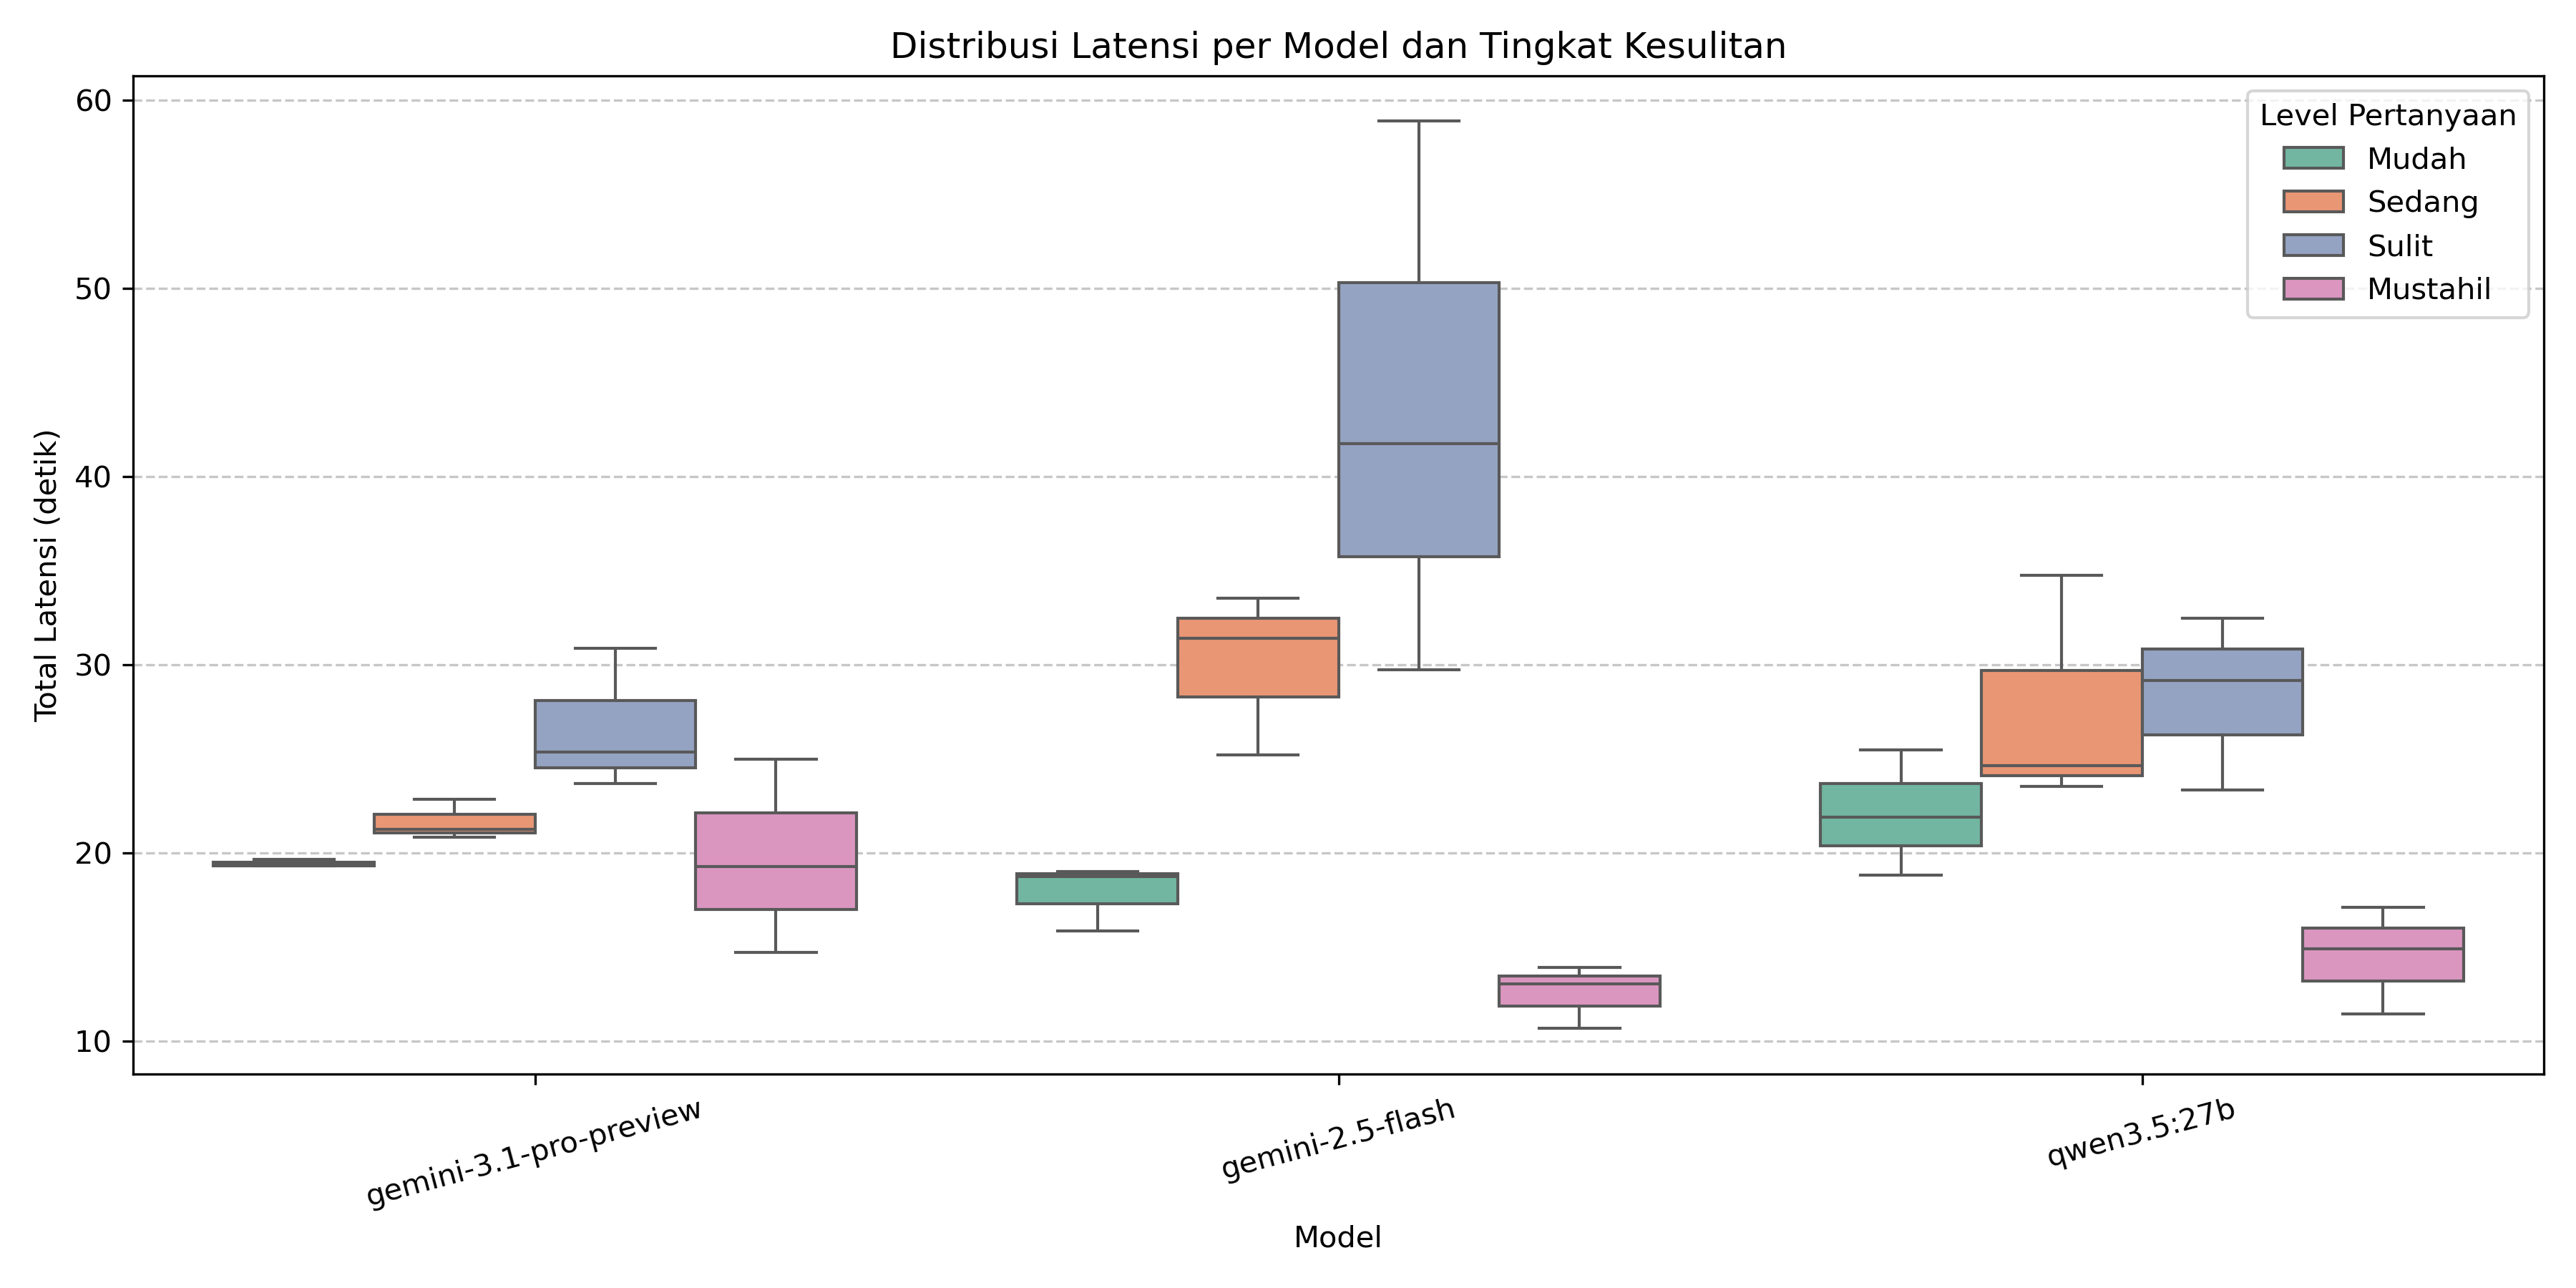
\includegraphics[width=\columnwidth]{figures/boxplot_plan_latensi.png}
\caption{Latency distribution for route planning evaluation. Gemini 2.5 Flash shows a latency spike on complex tasks due to excessive Chain-of-Thought generation.}
\label{fig:boxplot_plan}
\end{figure}

A notable trend reversal is shown in Fig.~\ref{fig:boxplot_plan}: Gemini 2.5 Flash, previously the fastest model, exhibited the highest latency and token consumption on complex planning tasks (spiking to $\sim$42s). This indicates that lightweight models require longer Chain-of-Thought scratchpads for high-level spatial reasoning, while Gemini 3.1 Pro's built-in reasoning engine solved routes more efficiently with fewer output tokens.

\subsection{End-to-End System Performance}
The full integration test comprised 9 scenarios across Easy (1 object), Medium (3 objects), and Hard (6 objects) levels, with each level including happy paths, anomaly paths, and HITL intervention paths. Four distinct operator intervention patterns were tested: initial plan alteration, mid-mission target addition, target cancellation and replacement, and manual secondary positioning. Evaluation metrics included plan success, route optimality, visual analysis accuracy, intervention handling, total session time, and token consumption.

\begin{table}[htbp]
\caption{Summary of End-to-End System Evaluation}
\label{tab:eval_e2e}
\centering
\resizebox{\columnwidth}{!}{%
\begin{tabular}{lccc}
\toprule
\textbf{Metric} & \textbf{Gemini 2.5 Flash} & \textbf{Gemini 3.1 Pro} & \textbf{Qwen 3.5 27B} \\
\midrule
Plan Success & 100.00\% & 100.00\% & 100.00\% \\
Route Optimality & 77.78\% & 100.00\% & 66.67\% \\
Visual Analysis & 86.67\% & 93.33\% & 63.33\% \\
Intervention Success & 100.00\% & 100.00\% & 100.00\% \\
Avg. Session Time (s) & 382.91 & 367.40 & 610.79 \\
Avg. Consumed Tokens & 153,564 & 183,440 & 140,072 \\
\bottomrule
\end{tabular}%
}
\end{table}

All three models achieved 100\% plan creation and intervention handling success across all 4 tested intervention patterns, proving the MCP architecture's stability in converting text decisions to physical robot actions and its adaptability to mid-mission operator commands. The HITL mechanism proved highly effective: when operators interrupted missions to inject new targets or adjust postures, the webhook-paused agentic loop accepted the new prompt, queried new coordinates if needed, and resumed navigation without system restart.

Gemini 3.1 Pro maintained 100\% route optimality (9/9 scenarios) and the highest visual analysis accuracy (93.33\%, 28/30 points). Its two visual analysis failures were color misidentifications of a fire extinguisher tube due to dominant yellow label sticker pixels---a vulnerability shared across all models and inherent to current MLLM architectures. Qwen 3.5 experienced severe visual analysis degradation (63.33\%) in E2E scenarios, repeatedly producing false positives on spatially complex anomalies (e.g., failing to detect a fallen extinguisher or a detached hose).

\begin{figure}[htbp]
\centering
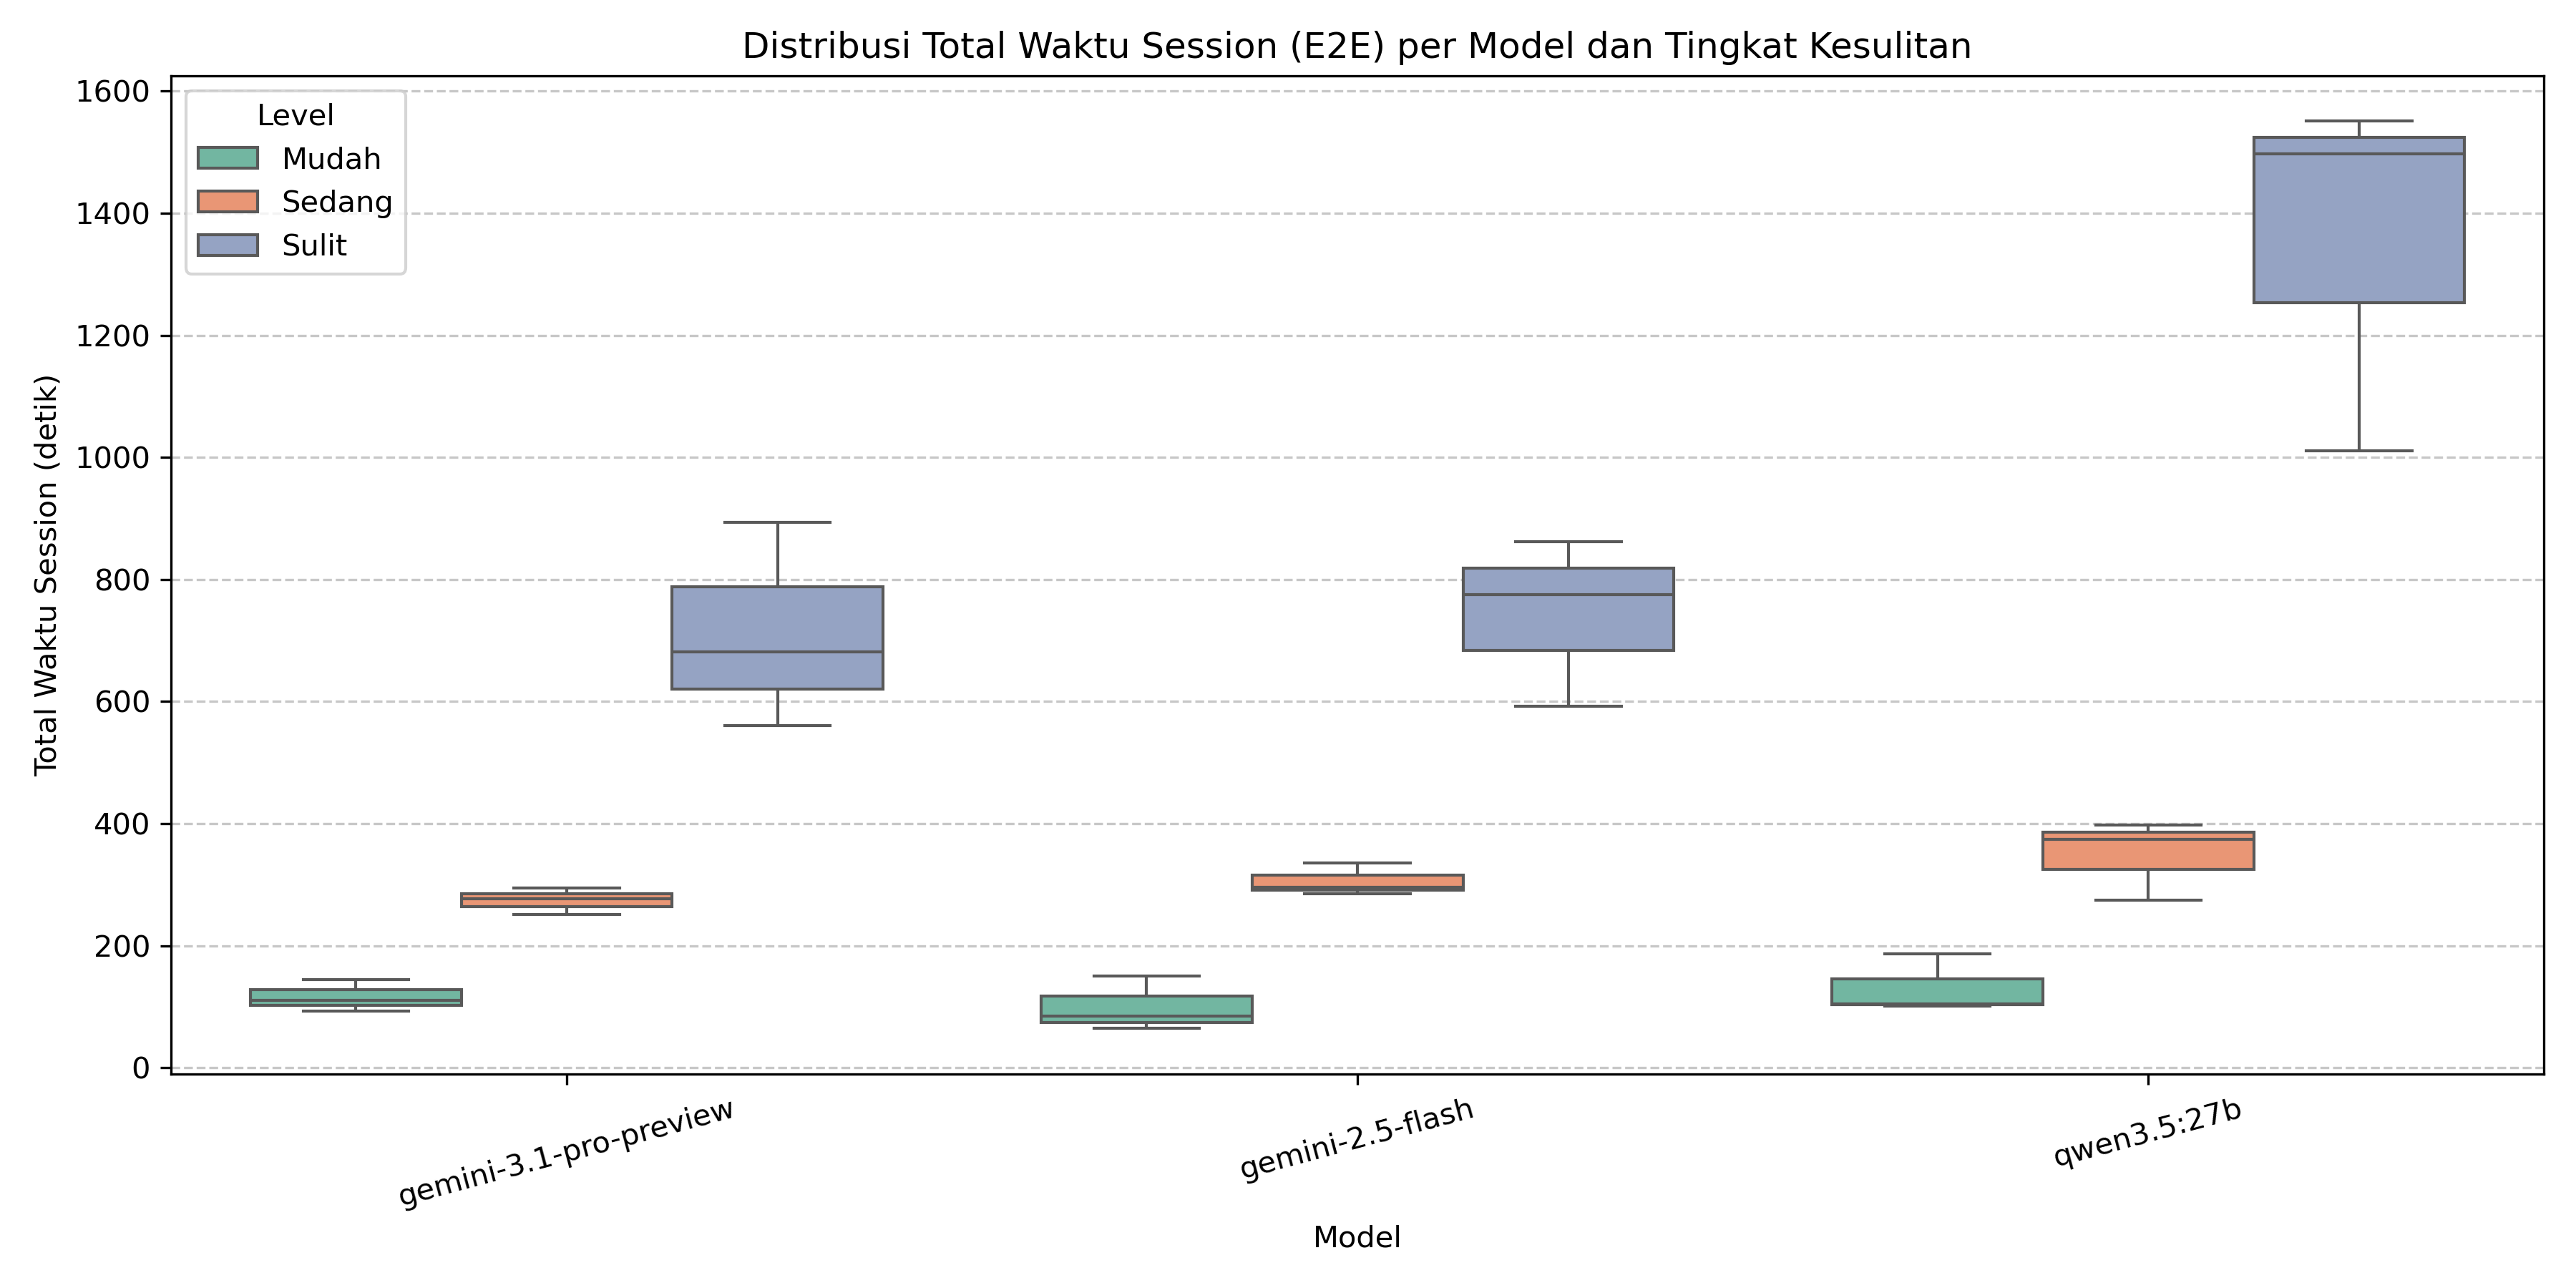
\includegraphics[width=\columnwidth]{figures/boxplot_e2e_latensi.png}
\caption{Session time distribution for E2E evaluation. Qwen 3.5 exhibits significantly higher session times at the Hard level (17--26 minutes) due to accumulated vision encoding overhead.}
\label{fig:boxplot_e2e}
\end{figure}

Session time analysis (Fig.~\ref{fig:boxplot_e2e}) revealed a counterintuitive latency anomaly between Gemini 2.5 Flash and Gemini 3.1 Pro. While Gemini 2.5 Flash demonstrated the fastest mission completion times in Easy scenarios, its session latency increased sharply in Medium and Hard levels, matching or slightly exceeding that of Gemini 3.1 Pro. Since plan generation occurs once at the start of a mission while visual analysis tool calls recur at every waypoint, Flash was expected to dominate overall mission speed based on isolated test results. Investigation indicates that this discrepancy was primarily driven by unequal network latency fluctuations between Flash and Pro API endpoints during testing. Meanwhile, Qwen 3.5 recorded the longest sessions at the Hard level (17--26 minutes), driven by compounding local visual feature extraction overhead across consecutive inspection targets.

\subsection{Operator Workload Assessment (NASA-TLX)}
A NASA Task Load Index survey with 10 respondents evaluated perceived operator workload across three conditions: fully manual teleoperation, autonomous navigation with manual visual analysis, and fully autonomous inspection. Results showed a consistent reduction in weighted workload scores: from 54.13 (High) for manual operation, to 34.57 (Medium) for autonomous navigation, to 18.40 (Low) for fully autonomous inspection. The primary workload reduction sources were Physical Demand (delegating navigation to ROS) and Mental Demand (delegating visual analysis to the MLLM). Individual anomalies where workload increased under automation were attributed to system malfunctions eroding trust and the psychological discomfort of transitioning from active controller to passive supervisor.

% ─────────────────────────────────────────────────────────
\section{Conclusion}

This paper presented an agentic AI-driven quadruped robot inspection system integrating Multimodal Large Language Models (MLLMs) with Human-in-the-Loop supervisory control. By combining the Model Context Protocol (MCP) for structured tool invocation, webhook-driven asynchronous execution callbacks, and Agentic RAG operational grounding, the system translates natural language instructions into physical robot navigation and SOP-based visual compliance analysis without code modifications.

Experimental evaluation across 9 end-to-end mission scenarios comprising 30 inspection points yielded key findings aligned with the research objectives:
\begin{enumerate}
    \item \textbf{MLLM Integration Performance:} Cloud-based Gemini 3.1 Pro Preview demonstrated superior performance, achieving 93.33\% (28/30) visual analysis accuracy, 100\% (9/9) route efficiency, and an average session time of 6.1 minutes. Gemini 2.5 Flash achieved 86.67\% (26/30) visual accuracy, 77.78\% (7/9) route efficiency, and 6.4 minutes average session time. Local model Qwen 3.5 27B recorded 63.33\% (19/30) visual accuracy, 66.67\% (6/9) route efficiency, and the highest session latency (10.2 minutes average, spiking up to 17--26 minutes on complex levels due to local vision encoding bottlenecks). Overall, MLLM deployment significantly reduced operator workload (NASA-TLX) from 54.13 (manual teleoperation) to 18.40 (fully autonomous inspection).
    \item \textbf{HITL Stepwise Adaptability:} The stepwise execution architecture with automated feedback enabled dynamic mid-mission adaptability. All tested models achieved 100\% success across four intervention patterns: initial plan alteration, mid-mission target addition, target cancellation and replacement, and manual secondary positioning.
\end{enumerate}

Future research will focus on: (1) implementing context pruning and memory summarization to stabilize local MLLM inference speed; (2) evaluating specialized Vision-Language Navigation (VLN) models (e.g., Qwen-RobotNav) for enhanced spatial reasoning; (3) migrating to ROS 2 Humble for advanced navigation stacks; and (4) expanding evaluation across broader environmental complexities and intervention variations.

% ─────────────────────────────────────────────────────────
\bibliographystyle{IEEEtran}
\begin{thebibliography}{00}

\bibitem{GrandView2024}
Grand View Research, ``Autonomous Mobile Robot Market Size, Share \& Trends Analysis Report,'' 2024. [Online]. Available: https://www.grandviewresearch.com

\bibitem{fan2024review}
J. Fan et al., ``A review of quadruped robots and environment perception,'' \textit{Sensors}, vol. 24, no. 4, 2024.

\bibitem{rea2022still}
D. Rea and C. Anagnostopoulos, ``Is teleoperation still relevant for human-robot interaction?'' \textit{ACM/IEEE HRI}, 2022.

\bibitem{Darmawan2025}
Darmawan, ``Pengembangan Robot Quadruped untuk Estimasi Posisi Komponen Overheat Pada Gardu Induk Berbasis Kamera Termal,'' Tugas Akhir, Institut Teknologi Sepuluh Nopember, 2025.

\bibitem{Mahendra2024}
V. G. P. A. B. Mahendra, ``Interaksi Robot Manusia Berbasis Large Language Model untuk Pembuatan Movement Plan pada Robot Quadruped-legged,'' Proposal Tugas Akhir, ITS, 2024.

\bibitem{huang2022language}
W. Huang et al., ``Language models as zero-shot planners: Extracting actionable knowledge for embodied agents,'' \textit{ICML}, 2022.

\bibitem{ravichandar2020recent}
H. Ravichandar et al., ``Recent advances in robot learning from demonstration,'' \textit{Annual Review of Control, Robotics, and Autonomous Systems}, vol. 3, 2020.

\bibitem{ahn2022do}
M. Ahn et al., ``Do as I can, not as I say: Grounding language in robotic affordances,'' \textit{arXiv:2204.01691}, 2022.

\bibitem{driess2023palm}
D. Driess et al., ``PaLM-E: An embodied multimodal language model,'' \textit{ICML}, 2023.

\bibitem{lewis2020retrieval}
P. Lewis et al., ``Retrieval-augmented generation for knowledge-intensive NLP tasks,'' \textit{NeurIPS}, 2020.

\bibitem{rosmann2012trajectory}
C. R{\"o}smann et al., ``Trajectory modification considering dynamic constraints of autonomous robots,'' \textit{ROBOTIK}, 2012.

\bibitem{biber2003normal}
P. Biber and W. Stra{\ss}er, ``The normal distributions transform: A new approach to laser scan matching,'' \textit{IROS}, 2003.

\bibitem{koide2021voxelized}
K. Koide et al., ``Voxelized GICP for fast and accurate 3D point cloud registration,'' \textit{ICRA}, 2021.

\bibitem{DEEPRoboticsLite3Pro2024}
DEEPRobotics, \textit{Jueying Lite3 Pro User Manual}, V1.0.7-0, 2024.

\bibitem{DEEPRoboticsLite3LiDAR2025}
DEEPRobotics, \textit{Jueying Lite3 LiDAR User Manual}, V1.0.7-0, 2025.

\bibitem{quigley2009ros}
M. Quigley et al., ``ROS: an open-source robot operating system,'' \textit{ICRA Workshop on Open Source Software}, 2009.

\end{thebibliography}

\end{document}
